\begin{figure}[t]
\centering
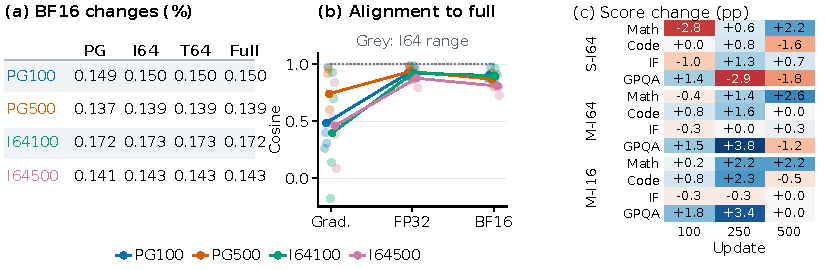
\includegraphics[width=\linewidth]{figures/table1_sync_20260918/section5_supervision.pdf}
\caption{\textbf{I64 better approximates the full-vocabulary gradient, with similar BF16 update sparsity and mixed task gains.}
(a) Nonzero BF16 changes (\%): rows are joint student/update, columns are local losses; colors also identify (b).
(b) Cosine to the full-vocabulary gradient or update; shading shows the I64 range.
(c) I64/I16 minus PG scores (percentage points), grouped by single-teacher I64, joint I64, and joint I16 training.}
\label{fig:supervision_overview}
\end{figure}
